\section{Theorie}
\label{sec:Theorie}
\subsection{Allgemein}
Trifft Licht auf einen Spalt oder ein kleines undurchlässiges Hinderniss, so weicht das Bild von den Gesetzen der geometrischen Optik ab.
Dies wird als Beugung des Lichtes bezeichnet.
Wird die Ausbreitung von Licht als klassische Welle beschrieben, so kann die Beugung erklärt werden.
Dabei wird der Teilchencharakter des Lichts vernachlässigt.

\subsection{Beugung an einem Parallelspalt}
Um Beugung am Spalt zu Untersuchen wird entweder die Fresnelsche oder die Frauenhofersche Lichtbeugung verwendet.
Bei der Fresnelschen Näherung wird von einem geringen Abstand zwischen Lichtquelle - Spalt und Spalt - Beobachtungspunkt $P$ ausgegangen.
Also interferieren Lichtstrahlen im Punkt $P$.
\\
Ist die Lichtquelle weit vom Spalt entfernt, so kann die Frauenhofersche Näherung verwendet werden.
Es wird außerdem angenommen, dass sich der Beobachtungspunkt $P$ im unendlichen befindet.
Das hat zu folge, dass alle Strahlen die in $P$ interferieren unter den gleichen Winkel $\phi$ gebeugt werden.
In Abb. \ref{fig:naeherung} ist die Fresnelsche und Frauenhofersche Beugung schematisch skizziert.
\begin{figure}
    \centering
    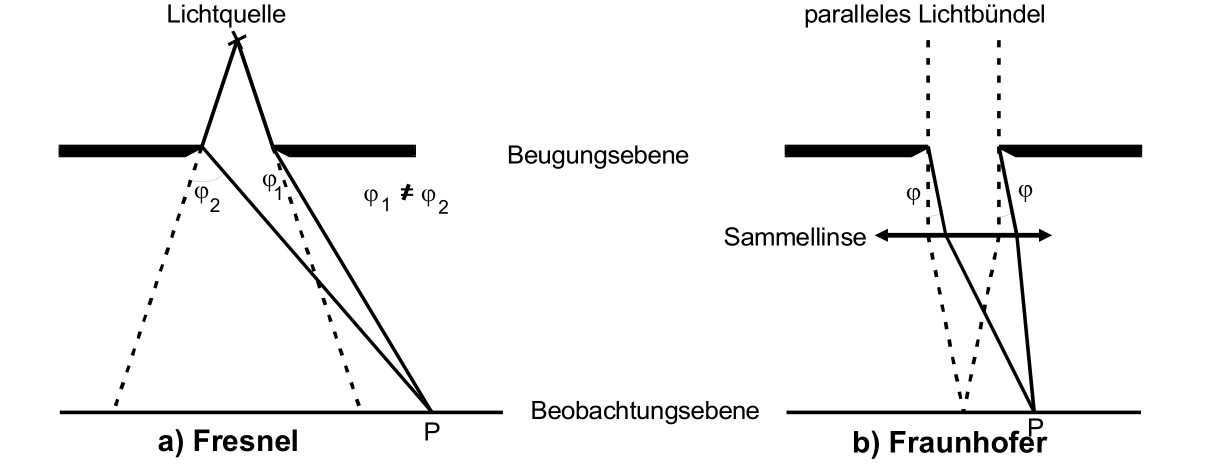
\includegraphics[width=0.8\textwidth]{content/data/naeherung.jpg}
    \caption{Die Fresnelsche (a) und Frauenhofersche Beugung (b) an einem Spalt. \cite[2]{anleitung}}
    \label{fig:naeherung}
\end{figure}
Ab hier wird nur die Frauenhofersche Beugung betrachtet.
Das erste Beugungsobjekt ist ein Spalt mit der Breite $b$ und einer Länge $l >> b$.
Das Licht wird also näherungsweise nur in einer Dimension begrenzt.
Die einfallende Welle hat die Feldstärke
\begin{equation*}
    A(z,t) = A_0 \cdot \mathrm{e}^{i(\omega t - \frac{2 \pi z}{\lambda})}
\end{equation*}
pro Längeneinheit der Wellenfront aus z-Richtung.
In dem Versuch wird als Lichtquelle ein Laser verwedet.
Die Entfernung zum Beobachtungspunkt $P$ ist groß zur Spaltbreite $b$.
\\
Das Huygenssche Prinzip besagt, dass jeder Punkt einer Wellenfront eine Elementarwelle aussendet.
Diese haben die Form einer Kugelwelle und interferieren miteinander und erzeugen eine neue Wellenfront.
Die Wellenfront entspricht der Einhüllenden der Elementarwellen.
Trifft Licht also durch den Spalt, so kann es sich nicht nur in die ursprüngliche Richtung ausbreiten, sondern sendet von jedem Punkt der Spaltöffnung eine Kugelwelle aus.
Zwei Strahlenbündel haben einen Phasenunterschied von
\begin{equation}
    \delta = \frac{2\pi x \sin (\phi)}{\lambda} .
\end{equation}
Die Breite $x$ zwischen den Strahlenbündel sind infinitesimal klein und es kann über die gesamte Spaltbreite integriert werden:
\begin{align*}
    B(z,t,\phi) = A_0 \int_0^b \mathrm{e}^{i(\omega t - \frac{2 \pi z}{\lambda} + \delta)} \mathrm{d}x \\
   = A_0 \mathrm{e}^{i \left (\omega t - \frac{2 \pi z}{\lambda} \right )} \cdot \mathrm{e}^{\frac{\pi i b \sin \phi}{\lambda}} \cdot \frac{\lambda}{\pi \sin \phi} \sin \left (\frac{\pi b \sin \phi}{\lambda} \right )
\end{align*}
